\documentclass[11pt]{aghdpl}
% \documentclass[en,11pt]{aghdpl}  % praca w języku angielskim

% Lista wszystkich języków stanowiących języki pozycji bibliograficznych użytych w pracy.
% (Zgodnie z zasadami tworzenia bibliografii każda pozycja powinna zostać utworzona zgodnie z zasadami języka, w którym dana publikacja została napisana.)
\usepackage[english,polish]{babel}

% Użyj polskiego łamania wyrazów (zamiast domyślnego angielskiego).
\usepackage{polski}

\usepackage[utf8]{inputenc}

% dodatkowe pakiety

\usepackage{mathtools}
\usepackage{amsfonts}
\usepackage{amsmath}
\usepackage{amsthm}

% --- < bibliografia > ---
\usepackage[
style=numeric,
sorting=none,
%
% Zastosuj styl wpisu bibliograficznego właściwy językowi publikacji.
language=autobib,
autolang=other,
% Zapisuj datę dostępu do strony WWW w formacie RRRR-MM-DD.
% urldate=iso,
% Nie dodawaj numerów stron, na których występuje cytowanie.
backref=false,
% Podawaj ISBN.
isbn=true,
% Nie podawaj URL-i, o ile nie jest to konieczne.
url=false,
%
% Ustawienia związane z polskimi normami dla bibliografii.
maxbibnames=3,
% Jeżeli używamy BibTeXa:
backend=bibtex
]{biblatex}

\usepackage{csquotes}
% Ponieważ `csquotes` nie posiada polskiego stylu, można skorzystać z mocno zbliżonego stylu chorwackiego.
\DeclareQuoteAlias{croatian}{polish}

\addbibresource{bibliografia.bib}

% Nie wyświetlaj wybranych pól.
%\AtEveryBibitem{\clearfield{note}}


% ------------------------
% --- < listingi > ---

% Użyj czcionki kroju Courier.
\usepackage{courier}

\usepackage{listings}
\lstloadlanguages{TeX}

\lstset{
	literate={ą}{{\k{a}}}1
           {ć}{{\'c}}1
           {ę}{{\k{e}}}1
           {ó}{{\'o}}1
           {ń}{{\'n}}1
           {ł}{{\l{}}}1
           {ś}{{\'s}}1
           {ź}{{\'z}}1
           {ż}{{\.z}}1
           {Ą}{{\k{A}}}1
           {Ć}{{\'C}}1
           {Ę}{{\k{E}}}1
           {Ó}{{\'O}}1
           {Ń}{{\'N}}1
           {Ł}{{\L{}}}1
           {Ś}{{\'S}}1
           {Ź}{{\'Z}}1
           {Ż}{{\.Z}}1,
	basicstyle=\footnotesize\ttfamily,
}

% ------------------------

\AtBeginDocument{
	\renewcommand{\tablename}{Tabela}
	\renewcommand{\figurename}{Rys.}
}

% ------------------------
% --- < tabele > ---

\usepackage{array}
\usepackage{tabularx}
\usepackage{multirow}
\usepackage{booktabs}
\usepackage{makecell}
\usepackage[flushleft]{threeparttable}

% defines the X column to use m (\parbox[c]) instead of p (`parbox[t]`)
\newcolumntype{C}[1]{>{\hsize=#1\hsize\centering\arraybackslash}X}


%---------------------------------------------------------------------------

\author{Mateusz Grzeliński, Agata Sidło, Kasia Lambrecht, Kasia Wilczak}
\shortauthor{M. Grzeliński, A. Sidło, K. Lambrecht, K. Wilczak}

\titlePL{Dokumentacja projektowa - automatyczny parking}
\titleEN{}
\shorttitlePL{}
\thesistype{Analiza i modelowanie oprogramowania}
\degreeprogramme{Informatyka}
\date{2018}
\department{Katedra Informatyki Stosowanej}
\faculty{Wydział Elektrotechniki, Automatyki,\protect\\[-1mm] Informatyki i Inżynierii Biomedycznej}
\acknowledgements{}


\setlength{\cftsecnumwidth}{10mm}

%---------------------------------------------------------------------------
\setcounter{secnumdepth}{4}
\brokenpenalty=10000\relax

\begin{document}

\titlepages

% Ponowne zdefiniowanie stylu `plain`, aby usunąć numer strony z pierwszej strony spisu treści i poszczególnych rozdziałów.
\fancypagestyle{plain}
{
        % Usuń nagłówek i stopkę
        \fancyhf{}
        % Usuń linie.
        \renewcommand{\headrulewidth}{0pt}
        \renewcommand{\footrulewidth}{0pt}
}

\setcounter{tocdepth}{2}
\tableofcontents
\clearpage

\chapter{Ogólny opis systemu}
\label{cha:wprowadzenie}


\section{Cel (przeznaczenie) systemu}
\label{sec:celePracy}

Celem systemu automatyczny parking jest umożliwienie komputerowej obsługi pobierania opłat za~pozostawienie pojazdu na parkingu na określony czas. System rozpoznaje ze zdjęcia tablice rejestracyjne pojazdów i na tej podstawie umożliwia wjazd samochodów na parking, a także opuszczenie go.

\section{Udziałowcy i użytkownicy}

\begin{list}{$\bullet$}{}
\item Właściciel - posiada parking, jest kierownikiem zarządzającym pracownikami, system prezentuje mu zebrane statystki
\item Klient - osoba, która korzysta z usług automatycznego parkingu i wjeżdza samochodem na jego teren
\item Operator - osoba kontrolująca parking w danej chwili, w przypadku błędów, przegląda zarejestrowane zdjęcia i poprawia czas wjazdu/wyjazdu, wprowadza rejestrację pojazdu do systemu oraz w~wyjątkowych sytuacjach podnosi/opuszcza szlaban

\end{list}

\section{Podstawowe cele udziałowców i użytkowników}

\begin{table}[H]
	\begin{tabular}{|l|l|l|} \hline
	\textbf{Udziałowcy}	& \textbf{Cel} & \textbf{Priorytet} \\ \hline% \bottomrule
	Klient	& Wjechanie na parking & Wysoki \\
	Klient	& Opuszczenie parkingu & Wysoki \\
	Klient	& Wpisanie numeru rejestracyjnego & Wysoki \\
	Klient	& Potwierdzenie zdjęcia & Wysoki \\
	Klient	& Anulowanie wpisanego numeru rejestracyjnego & Średni \\
	Klient	& Uiszczenie opłaty & Wysoki \\
	Operator& Przeglądanie zdjęć & Średni \\
	Operator& Wprowadzenie rejestracji & Średni \\
	Operator& Poprawa czasu wjazdu i wyjazdu w bazie & Średni \\
	Operator& Podnoszenie/opuszczanie szlabanu & Średni \\
	Właściciel& Wyświetlenie statystyk & Niski \\ \hline
	\end{tabular}
\end{table}

\subsection{Porównanie proponowanego systemu do aktualnie funkcjonującego}
%płatność kartą i gotówką?
Na parkingu znajdującym się koło Wawelu w Krakowie klient podjeżdża do terminala, naciska przycisk i~odbiera bilet z godziną wjazdu. Przy opuszczaniu parkingu wkłada otrzymany przy wjeździe bilet i~dokonuje opłaty.
W~naszym systemie klient, wjeżdżając na parking, nie musi podjeżdżać do terminala i~czekać na wydrukowanie kartki z~godziną wjazdu. System zrobi zdjęcie tablicy rejestracyjnej i~sam otworzy szlaban. W~ten sposób oszczędzany jest papier oraz tusz. Operator nie musi dbać o~to żeby ich nie zabrakło. Musi jedynie interweniować w~przypadku błędu.


\section{Granice systemu}
\begin{figure}[H]
	\centering
	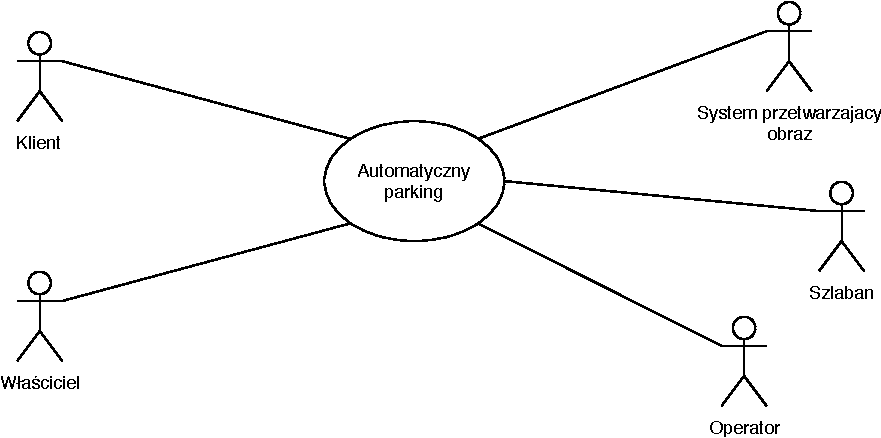
\includegraphics[width=90mm]{diagramy/graniceSystemu.pdf}
	\caption{Granice systemu automatyczny parking \label{overflow}}
\end{figure}

\section{Lista funkcji systemu}


\begin{enumerate}
	\item Wykrycie pojawienia się pojazdu
	\item Zapis zdjęcia rejestracji
	\item Zapis tablicy rejestracyjnej
	\item Otwarcie szlabanu
	\item Zamknięcie szlabanu
	\item Wyświetlenie zdjęcia tablicy rejestracyjnej
	\item Obliczenie kwoty do zapłaty
	\item Wyświetlenie kwoty do zapłaty
	\item Oczekiwanie na pojazd do 15 minut
	\item Zgłoszenie niezgodności wpisanej i zarejestrowanej rejestracji
	\item Wyświetlenie wpisanego przez klienta numeru rejestracyjnego
	\item Zapis danych
	\item Prezentacja statystyk
\end{enumerate}

\section{Diagramy czynności}

% Diagram czynności: Klient wjeżdża na parking
\begin{figure}[H]
	\centering
	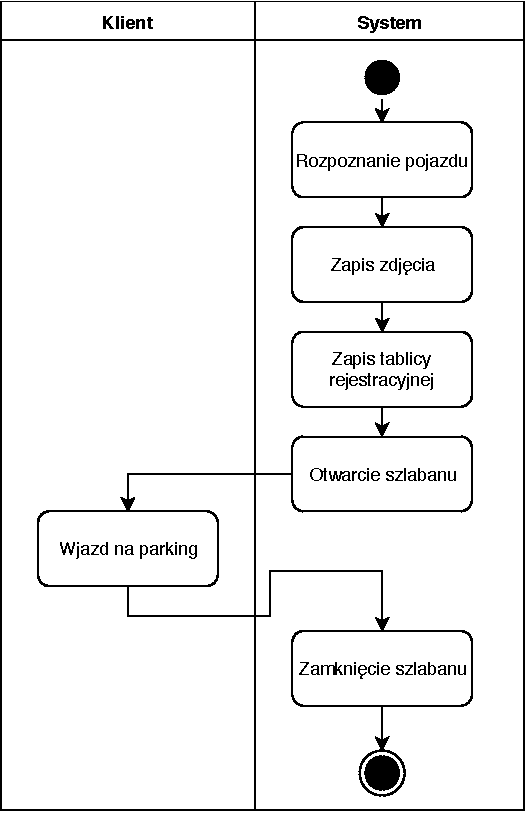
\includegraphics[width=90mm]{diagramy/DiagCzynWjazd.pdf}
	\caption{Diagram czynności: Klient wjeżdża na parking \label{overflow}}
\end{figure}


% Diagram czynności: Klient opuszcza parking
\begin{figure}[H]
	\centering
	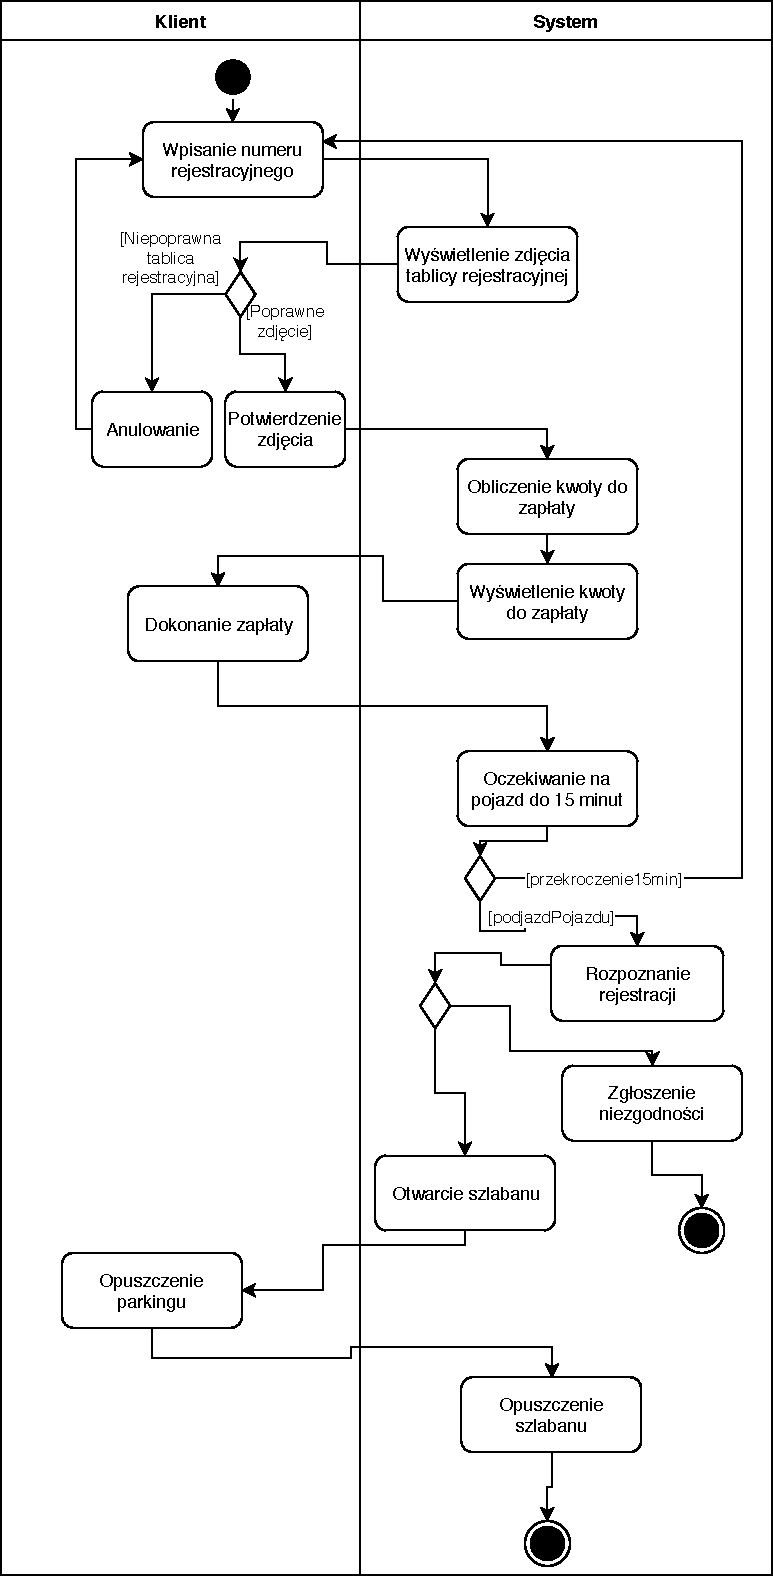
\includegraphics[width=90mm]{diagramy/DiagCzynWyjazd.pdf}
	\caption{Diagram czynności: Klient opuszcza parking \label{overflow}}
\end{figure}


% Diagram czynności: Operator weryfikuje wykryte oszustwo
\begin{figure}[H]
	\centering
	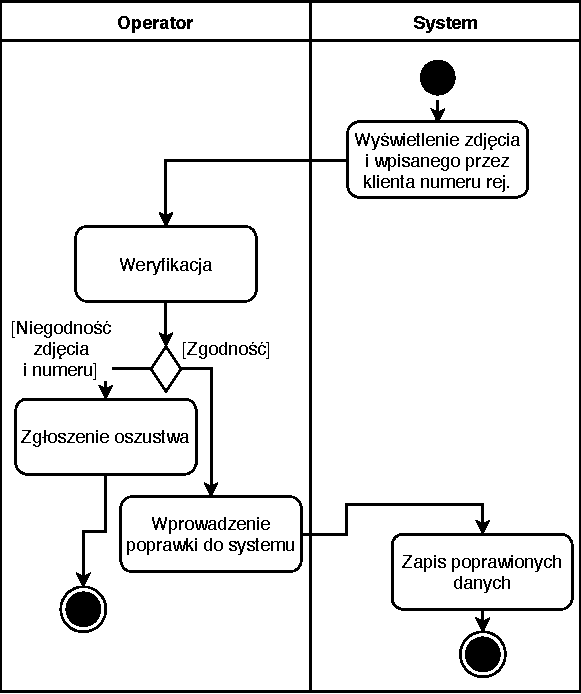
\includegraphics[width=90mm]{diagramy/DiagCzynWyswietlZdjecia.pdf}
	\caption{Diagram czynności: Operator weryfikuje wykryte oszustwo \label{overflow}}
\end{figure}

% Diagram czynnosci: Właściciel wyświetla statystyki
\begin{figure}[H]
	\centering
	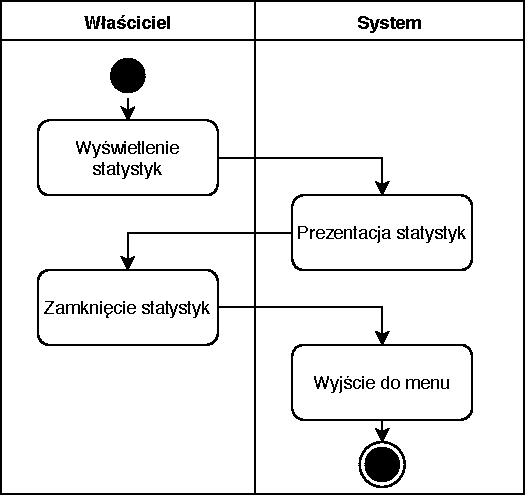
\includegraphics[width=90mm]{diagramy/DiagCzynStatystyki.pdf}
	\caption{Diagram czynności: Właściciel wyświetla statystyki \label{overflow}}
\end{figure}





\chapter{Analiza Dziedziny}
\label{cha:anDziedziny}
%---------------------------------------------------------------------------

\section{Klasy i opis atrybutów}
\label{sec:klasyAtrybuty}
\begin{table}[H]
	\begin{tabular}{|l|l|l|} \hline
	\textbf{Klasa}	& \textbf{Atrybut} & \textbf{Opis} \\ \hline% \bottomrule
	Pojazd	& NumerRejestracyjny & Numer rejestracyjny pojazdu \\
	& Marka & Marka pojazdu \\
	& Model & Model pojazdu \\
	Samochód& & \\
	Motor& &  \\
	Autobus& & \\
	Parking	& IloscWolnychMiejsc & Określa ilość wolnych miejsc na parkingu \\
	MiejsceParkingowe	& Numer & Numer miejsca parkingowego \\
	& Typ & Typ miejsca parkingowego \\
	& Status & Określa status miejsca - wolne/zajęte \\
	Wjazd	& DataWjazdu & Data wjazdu na parking\\
	& CzasWjazdu & Czas wjazdu na parking \\
	& Pojazd & Określa pojazd, którego dotyczy wjazd \\
	Wyjazd	& DataWyjazdu & Data wyjazdu z parkingu\\
	& CzasWyjazdu & Czas wjazdu z parkingu \\
	& Pojazd & Określa pojazd, którego dotyczy wyjazd \\
	& StatusPlatnosci & Określa, czy płatność została zrealizowana \\
	Terminal & Status & Status określa możliwość wjazdu/wyjazdu na/z parkingu \\
	Szlaban & Status & Określa, czy szlaban jest otwarty/zamknięty\\
	Operator& Id & Id operatora \\
	& Imię & Imię operatora \\
	& Nazwisko & Nazwisko operatora \\
	BazaZdjęć& &  \\ \hline
	\end{tabular}
\end{table}


%---------------------------------------------------------------------------

\section{Diagramy klas  - relacje}
\label{sec:diagKlas}
% Diagram klas
\begin{figure}[H]
	\centering
	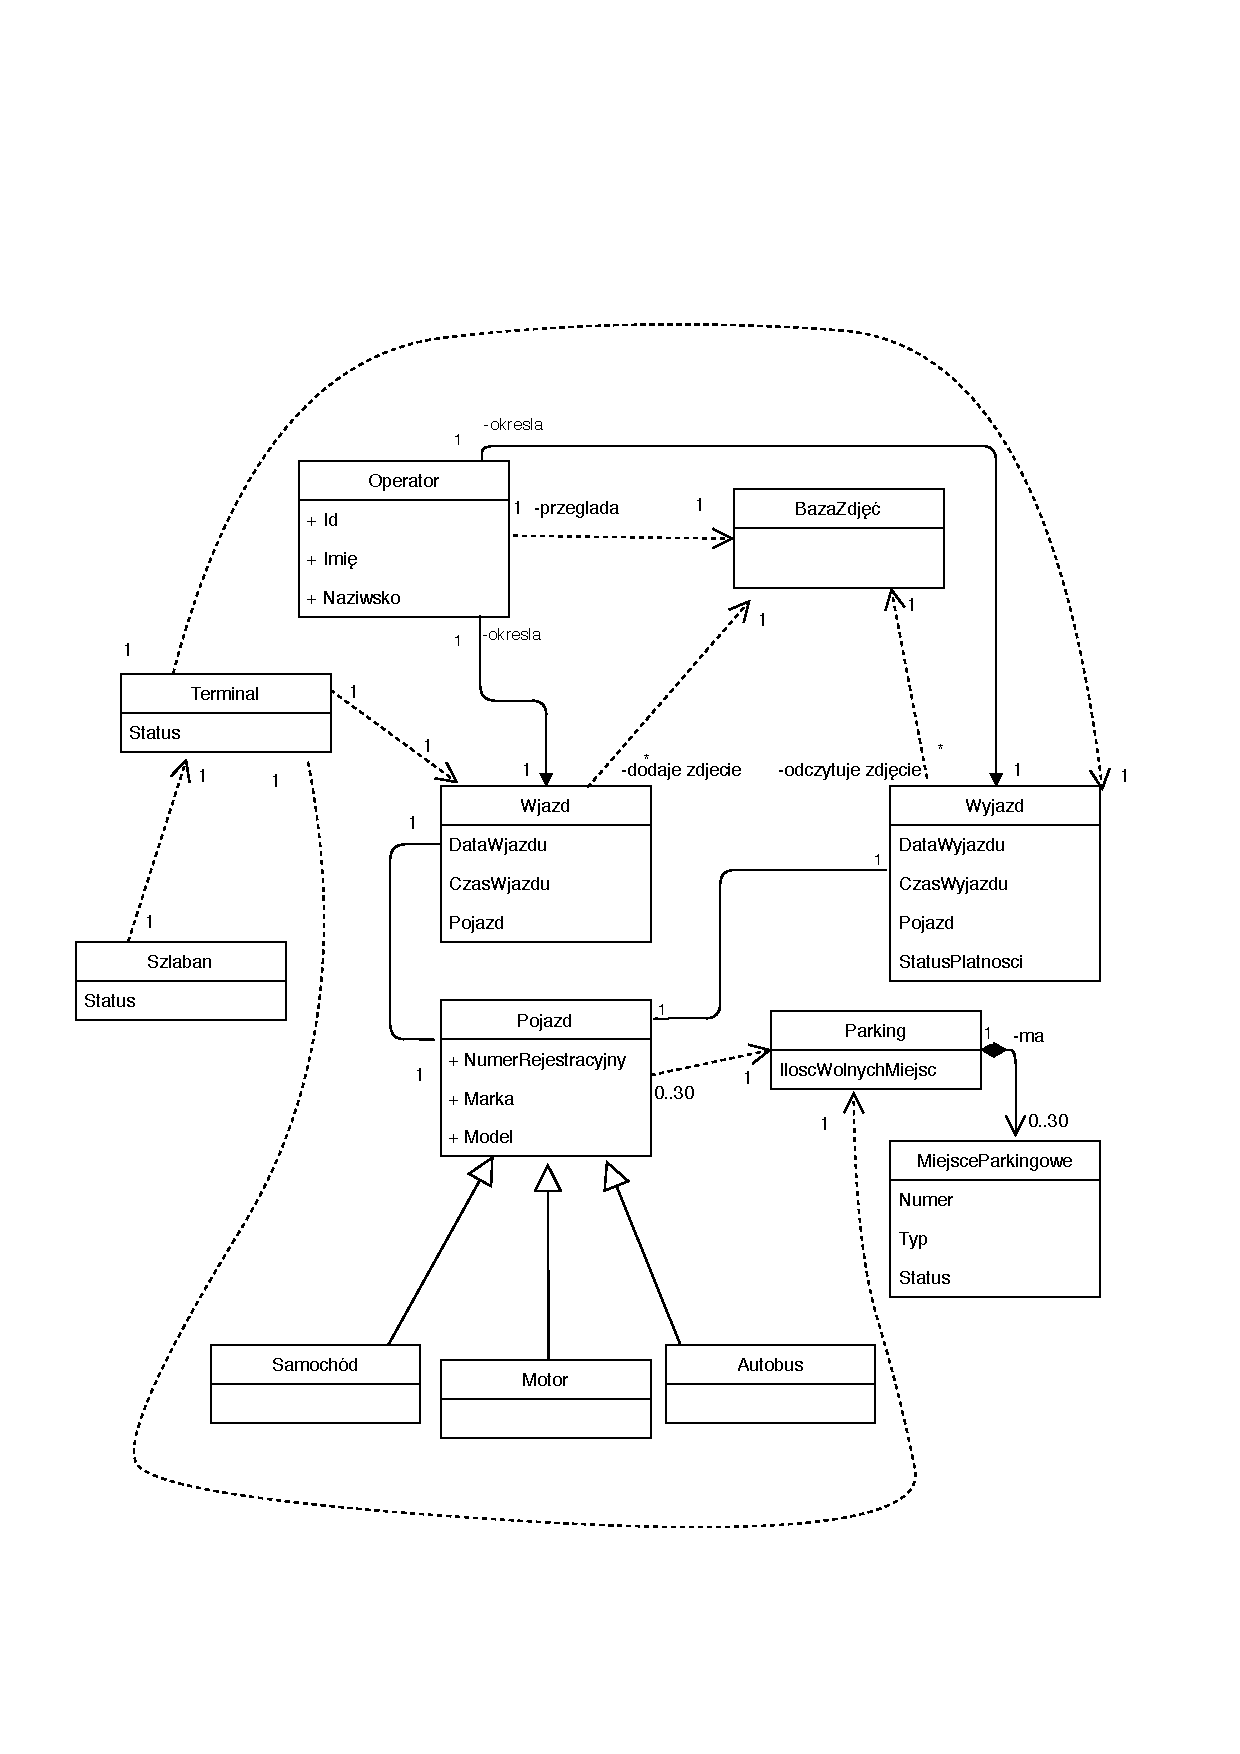
\includegraphics[width=150mm]{diagramy/DiagKlas.pdf}
	\caption{Diagram klas i relacje między nimi \label{overflow}}
\end{figure}


%---------------------------------------------------------------------------

\section{Diagramy stanów dla wybranych klas}
\label{sec:diagStanow}



%---------------------------------------------------------------------------

\section{Słownik pojęć}
\label{sec:slownik}


\chapter{SRS - specyfikacja wymagań}

\section{Ogólny diagram przypadków użycia}

\begin{figure}[H]
	\centering
	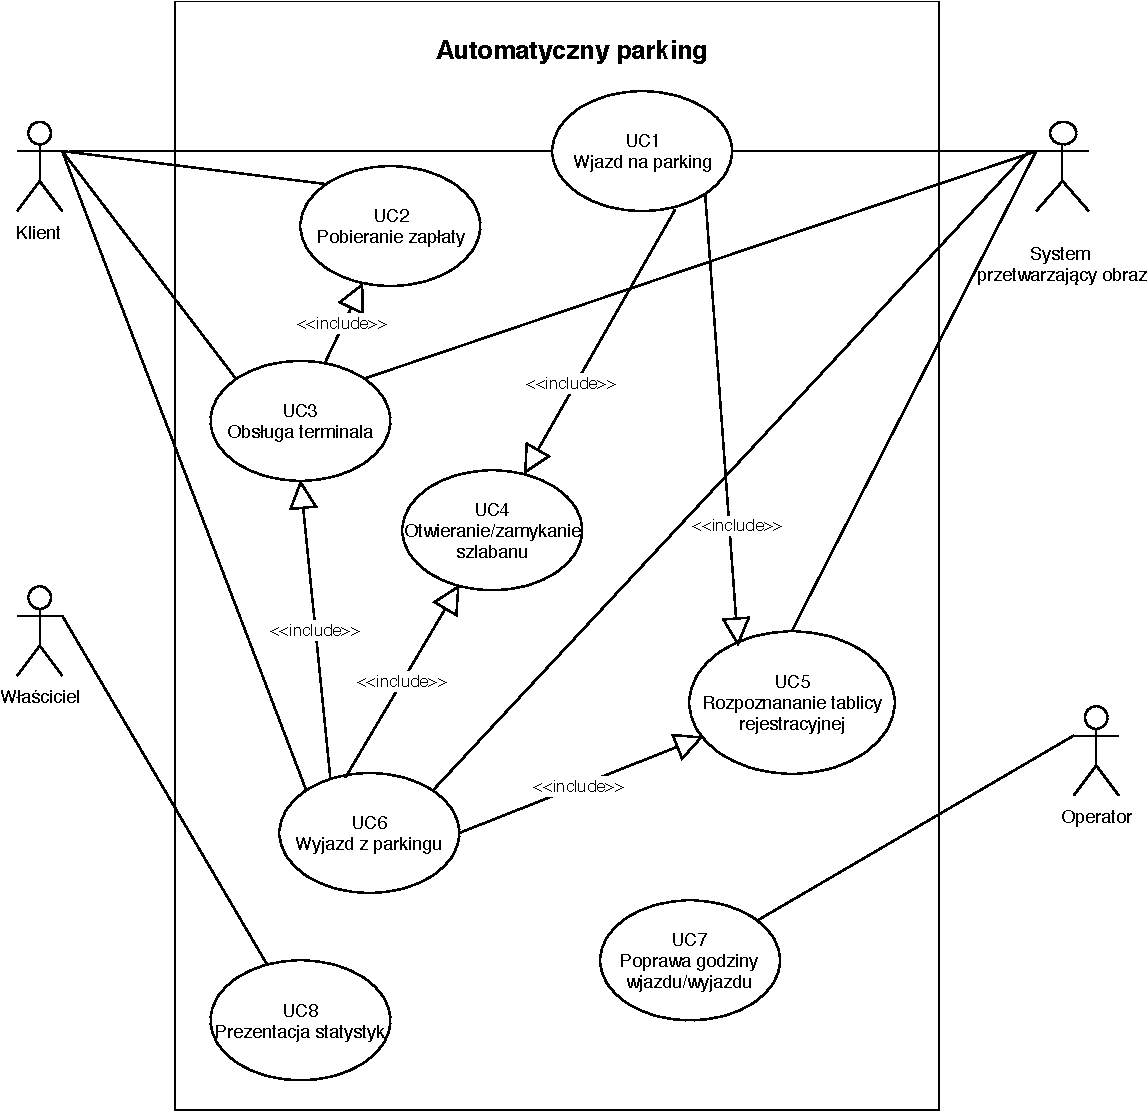
\includegraphics[width=100mm]{diagramy/PrzypUzycia.pdf}
	\caption{Przypadki użycia }
\end{figure}

\section{Definicje przypadków użycia}
\subsection{Obsługa terminala (identyfikator: UC3)}
\textbf{Aktorzy: }Klient, System przetwarzający obraz

\hspace{0cm}\textbf{Zakres: }System automatycznego parkingu

\hspace{0cm}\textbf{Poziom: }Systemowy

\hspace{0cm}\textbf{Udziałowcy i ich cele: }Klient chce dokonać zapłaty za postój, system musi pobrać wszystkie niezbędne dane oraz pobrać płatność

\hspace{0cm}\textbf{Zdarzenie wyzwalające (trigger): }Klienta wybiera funkcję Zapłać za postój

\hspace{0cm}\textbf{Warunki wstępne: }Tablica rejestracyjna pojazdu klienta musi znajdować się w systemie i być poprawnie odczytana

\hspace{0cm}\textbf{Warunki końcowe dla sukcesu: }
Tablica rejestracyjna zostaje potwierdzona przez klienta, płatność zostaje potwierdzona przez system

\hspace{0cm}\textbf{Warunki końcowe dla niepowodzenia: }Tablica rejestracyjna nie zostaje potwierdzona, płatność nie zostaje przetworzona \newline

\hspace{0cm}\textbf{Scenariusz główny: }
\begin{enumerate}
\item System wyświetla formularz wprowadzania rejestracji
\item Klient wprowadza rejestrację do systemu
\item System przetwarzający obraz weryfikuje wprowadzoną rejestrację
\item System wyświetla odpowiednią rejestrację
\item Klient potwierdza zdjęcie rejestracji
\item System wyświetla kwotę do zapłaty
\item Klient dokonuje zapłaty za postój
\item System przetwarza płatność (include UC2)
\item System wyświetla potwierdzenie zapłaty
\end{enumerate}
\hspace{0cm}\textbf{Scenariusz alternatywny: }
\begin{enumerate}
\item[3.a] Wprowadzona rejestracja nie zostaje znaleziona
\item[3.a.1] Następuje powrót do punktu 1 scenariusza głównego 
\end{enumerate}
\hspace{0cm}\textbf{Scenariusz alternatywny: }
\begin{enumerate}
	\item[5.a] Klient nie potwierdza zdjęcia rejestracji
	\item[5.a.1] Następuje powrót do punktu 1 scenariusza głównego
\end{enumerate}
\hspace{0cm}\textbf{Scenariusz alternatywny: }
\begin{enumerate}
\item[8.a] Płatność nie została przetworzona poprawnie
\item[8.a.1] Następuje powrót do punktu 6 scenariusza głównego 
\end{enumerate}
\subsection{Wjazd na parking (identyfikator: UC1)}
\textbf{Aktorzy: }System przetwarzający obraz, Szlaban

\hspace{0cm}\textbf{Zakres: } System automatycznego parkingu

\hspace{0cm}\textbf{Poziom: } Systemowy

\hspace{0cm}\textbf{Udziałowcy i ich cele: } Klient chce wjechać na parking, System przetwarzający obraz musi rozpoznać tablicę rejestracyjną

\hspace{0cm}\textbf{Zdarzenie wyzwalające (trigger): } Klient podjeżdza pojazdem pod szlaban

\hspace{0cm}\textbf{Warunki wstępne: } Tablica rejestracyjna pojazdu jest widoczna i możliwa do odczytania przez system przetwarzający obraz

\hspace{0cm}\textbf{Warunki końcowe dla sukcesu: }
System przetwarzający obraz poprawnie odczytuje tablicę rejestracyjną, szlaban otwiera się

\hspace{0cm}\textbf{Warunki końcowe dla niepowodzenia: } System przetwarzający obraz nie może odczytać tablicy rejestracyjnej, szlaban nie otwiera się \newline

\hspace{0cm}\textbf{Scenariusz główny: }
\begin{enumerate}
\item System przetwarzający obraz robi zdjęcie
\item System przetwarzający obraz odczytuje tablicę rejestracyjną
\item System automatycznego parkingu zapisuje datę i czas wjazdu pojazdu
\item Szlaban otwiera się (include: UC4)
\item Klient wjeżdża na parking
\item Szlaban zamyka się (include: UC4)
\end{enumerate}
\hspace{0cm}\textbf{Scenariusz alternatywny: }
\begin{enumerate}
\item[2.a] System przetwarzający obraz nie może odczytać tablicy rejestracyjnej
\item[2.a.1] Następuje powrót do punktu 1 scenariusza głównego
\end{enumerate}


\subsection{Wyjazd z parkingu (identyfikator: UC5)}
\textbf{Aktorzy: }System przetwarzający obraz, Szlaban

\hspace{0cm}\textbf{Zakres: }System automatycznego parkingu

\hspace{0cm}\textbf{Poziom: }Systemowy

\hspace{0cm}\textbf{Udziałowcy i ich cele: }Klient chce wyjechać z parkingu

\hspace{0cm}\textbf{Zdarzenie wyzwalające (trigger): } System odlicza 15 minut na wyjazd z parkingu

\hspace{0cm}\textbf{Warunki wstępne: }
Rejestracja pojazdu została poprawnie odczytana przy wjeździe

\hspace{0cm}\textbf{Warunki końcowe dla sukcesu: }Klient opuścił parking

\hspace{0cm}\textbf{Warunki końcowe dla niepowodzenia: }Klient nie opuścił parkingu \newline

\hspace{0cm}\textbf{Scenariusz główny: }
\begin{enumerate}
\item Klient obsługuje terminal (inlcude: UC3)
\item System potwierdza możliwość wyjazdu w ciągu 15 minut
\item System przetwarzający obraz ponownie robi zdjęcie
\item System przetwarzający obraz rozpoznaje tablicę rejestracyjną
\item System automatycznego parkingu weryfikuje dane: numer rejestracyjny, potwierdzenie płatności, pozostały czas wyjazdu
\item Szlaban otwiera się (include: UC4)
\item Klient opuszcza parking
\item Szlaban zamyka się (include: UC4)
\end{enumerate}
\hspace{0cm}\textbf{Scenariusz alternatywny: }
\begin{enumerate}
\item[4.a] System przetwarzający obraz nie może rozpoznać tablicy rejestracyjnej
\item[4.a.1] Następuje powrót do punktu 3 scenariusza głównego
\end{enumerate}

\hspace{0cm}\textbf{Scenariusz alternatywny: }
\begin{enumerate}
\item[5.a] Płatność nie została potwierdzona
\item[5.a.1] Następuje powrót do punktu 1 scenariusza głównego
\end{enumerate}

\hspace{0cm}\textbf{Scenariusz alternatywny: }
\begin{enumerate}
\item[5.a] Czas na wyjazd z parkingu skończył się
\item[5.a.1] Następuje powrót do punktu 1 scenariusza głównego
\end{enumerate}

\subsection{Prezentacja statystyk (identyfikator: UC8)}
\textbf{Aktorzy: }Właściciel

\hspace{0cm}\textbf{Zakres: }System automatycznego parkingu

\hspace{0cm}\textbf{Poziom: }systemowy

\hspace{0cm}\textbf{Udziałowcy i ich cele: } Właściciel chce wyświetlić statystyki

\hspace{0cm}\textbf{Zdarzenie wyzwalające (trigger): } Właściciel wywołuje funkcję Pokaż statystyki

\hspace{0cm}\textbf{Warunki wstępne: }
Właściciel musi być zalogowany

\hspace{0cm}\textbf{Warunki końcowe dla sukcesu: } System prezentuje wybrane statystyki

\hspace{0cm}\textbf{Warunki końcowe dla niepowodzenia: } System nie może wyświetlić wybranych statystyk, błędne dane \newline

\hspace{0cm}\textbf{Scenariusz główny: }
\begin{enumerate}
\item System wyświetla rodzaje statystyk do wyboru: dzienne, miesięczne, roczne
\item Właściciel wybiera odpowiedni rodzaj statystyk
\item System oblicza wybrane statystyki
\item System prezentuje wyniki
\end{enumerate}
\hspace{0cm}\textbf{Scenariusz alternatywny: }
\begin{enumerate}
\item[3.a] System nie może wyświetlić wybranych statystyk
\item[3.a.1] Właściciel poprawia błędne dane w systemie
\item[3.a.2] Następuje powrót do punktu 1 scenariusza głównego
\end{enumerate}

\subsection{Poprawa danych w systemie (identyfikator: UC7)}
\textbf{Aktorzy: }Operator

\hspace{0cm}\textbf{Zakres: }System automatycznego parkingu

\hspace{0cm}\textbf{Poziom: }Systemowy

\hspace{0cm}\textbf{Udziałowcy i ich cele: }Operator chce poprawić błędne dane w systemie

\hspace{0cm}\textbf{Zdarzenie wyzwalające (trigger): }Operator wywołuje funkcję Popraw dane

\hspace{0cm}\textbf{Warunki wstępne: }
Operator musi byc zalogowany

\hspace{0cm}\textbf{Warunki końcowe dla sukcesu: }Do systemu zostają wprowadzone poprawne dane

\hspace{0cm}\textbf{Warunki końcowe dla niepowodzenia: }System nie może przetworzyć nowych danych\newline

\hspace{0cm}\textbf{Scenariusz główny: }
\begin{enumerate}
\item System wyświetla formularz poprawiania danych
\item Operator wprowadza poprawione dane: numer rejestracyjny, godzinę wjazdu/wyjazdu, datę wjazdu/wyjazdu
\item System przetwarza wprowadzone dane
\item System wyświetla potwierdzenie zmian
\end{enumerate}

\hspace{0cm}\textbf{Scenariusz alternatywny: }
\begin{enumerate}
\item[3.a] system nie może przetworzyć nowych danych
\item[3.a.1] System wyświetla ponownie formularz, znaznaczając które pola zostały niepoprawnie wypełnione
\item[3.a.2] Następuje powrót do punktu 3 scenariusza głównego
\end{enumerate}

\chapter{Architektura systemu}

\section{Wyliczenie warstw lub wyliczenie podstawowych komponentów będących odrębnymi programami (nadawca-odbiorca, klient-serwer). Zamodelowanie ich jako klas z odpowiednim zestawem metod.}


\section{Specyfikacja interfejsu pomiędzy komponentami}

\chapter{Projekt oprogramowania}

\section{Sekcja..}

\chapter{Projekt interfejsu użytkownika IRS}

\section{Sekcja...}

\chapter{Projekt bazy danych}

\section{Projekt bazy}

\begin{figure}[H]
	\centering
	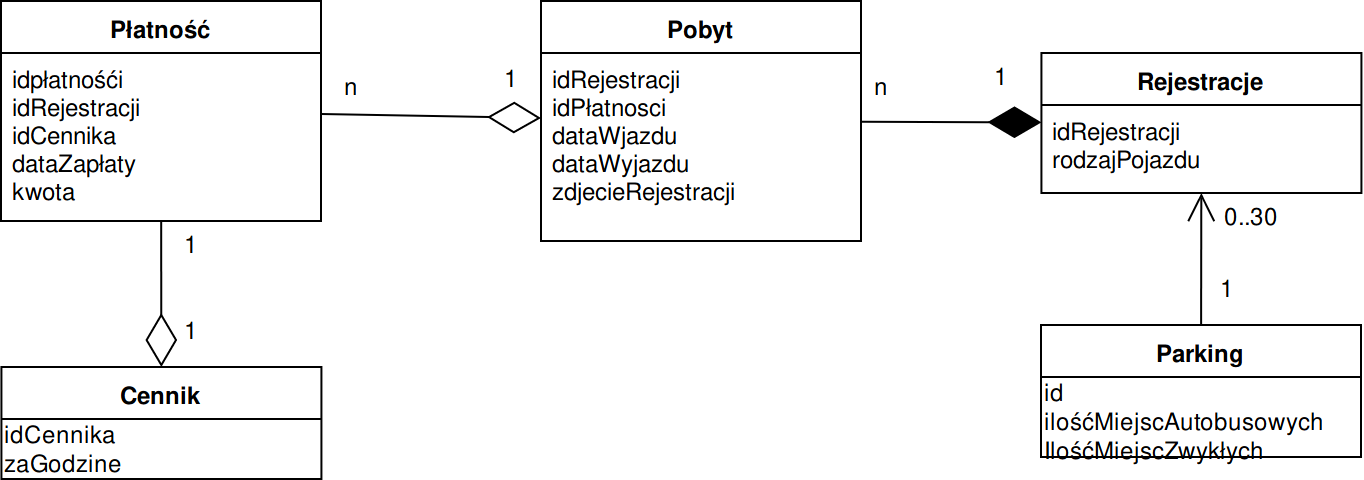
\includegraphics[width=140mm]{diagramy/bazaDanych.png}
  \caption{Projekt bazy danych}
\end{figure}



\section{Specyfikacja kwerend}


% itd.
% \appendix
% \include{dodatekA}
% \include{dodatekB}
% itd.

\printbibliography

\end{document}
